% Created 2021-08-02 seg 14:33
% Intended LaTeX compiler: pdflatex
\documentclass[11pt]{article}
\usepackage[utf8]{inputenc}
\usepackage[T1]{fontenc}
\usepackage{graphicx}
\usepackage{grffile}
\usepackage{longtable}
\usepackage{wrapfig}
\usepackage{rotating}
\usepackage[normalem]{ulem}
\usepackage{amsmath}
\usepackage{textcomp}
\usepackage{amssymb}
\usepackage{capt-of}
\usepackage{hyperref}
\author{Ruan Flaneto Cartier}
\date{\today}
\title{Projeto automação residencial}
\hypersetup{
 pdfauthor={Ruan Flaneto Cartier},
 pdftitle={Projeto automação residencial},
 pdfkeywords={},
 pdfsubject={},
 pdfcreator={Emacs 28.0.50 (Org mode 9.5)}, 
 pdflang={English}}
\begin{document}

\maketitle
\tableofcontents


\section{Motivação}
\label{sec:orgb9378d8}
Um projeto de automação residencial foi demandado. Primeira coisa que vem em mente é poder controlar as lâmdas de casa individualemente como meio de gerenciar o uso de cargas residenciais, viabilizando a economia de energia elétrica. Assim, pretende-se usar um módulo de ESP01 com relé (vide figura \ref{fig:module_esp01}) para cada ponto de interruptor de lâmpada para poder ter conexão com o computador central (raspberry pi).

\section{Objetivos}
\label{sec:org1356447}
Gerenciar o funcionamento das lâmpadas de casa, cujo funcionamento deve ser por comando de voz ou de forma manual. Este gerenciamento também inclui a formação de relatórios sobre consumo elétrico (estimado) em cada dispositivo, apresentando as informações em histogramas.

\section{Detalhamento do projeto}
\label{sec:org6ed61bc}
\subsection{Lâmpadas}
\label{sec:org1ab71dd}
\subsubsection{Descrição do circuito}
\label{sec:org7aaeb38}
Um pequeno trafo recebe a energia da tomada, é retificada por uma ponte retificadora e então o módulo relé com o esp8266 controla o chaveamento da lâmpada. Para fazer o controle da lâmpada ser manual torna-se necessário detectar a existência de fase no pino Normalmente Aberto (NA) do relé, como na figura \ref{fig:tomada}.

\begin{figure}[h!]
\caption{\label{fig:tomada}Circuito a ser implementado para detecção de fase}
\centering
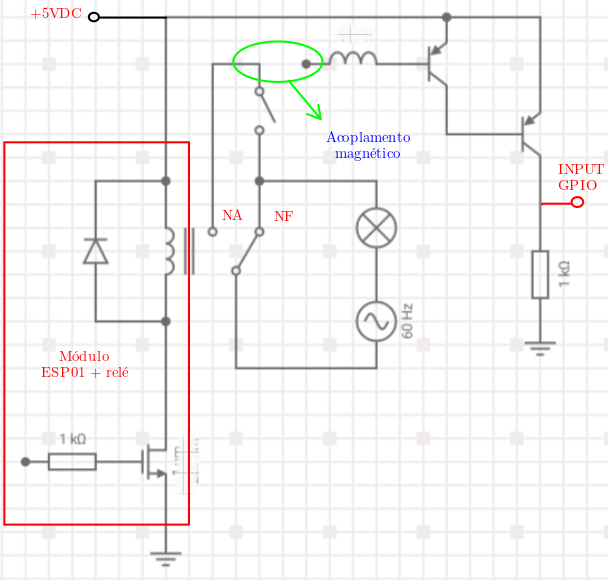
\includegraphics[width=0.7\textwidth]{./tomada.png}
\end{figure}

Não é intenção deste projeto confeccionar placa de circuito impresso para simplificar o projeto e também no momento é impossível para mim imprimir sem uma impressora adequada.
\subsubsection{Componentes utilizados (por lâmpada)}
\label{sec:org475f50f}
\begin{itemize}
\item[{$\boxtimes$}] 1 Trafo de carregador;
\item[{$\boxtimes$}] 4 Diodos 1n4007;
\item[{$\boxtimes$}] 1 Capacitor eletrolítico (47uF);
\item[{$\boxtimes$}] 1 Capacitor cerâmico (100nF);
\item[{$\boxtimes$}] 1 Sensor piroelétrico
\item[{$\boxtimes$}] 1 Módulo de acionamento de relé por ESP8266 (figura \ref{fig:module_esp01};
\item[{$\boxtimes$}] 2 transistores de uso geral para para detecção de fase;
\item[{$\boxtimes$}] Resistores diversos
\end{itemize}
\begin{figure}[h!]
\caption{\label{fig:module_esp01}Módulo relé com ESP01 utilizado}
\centering
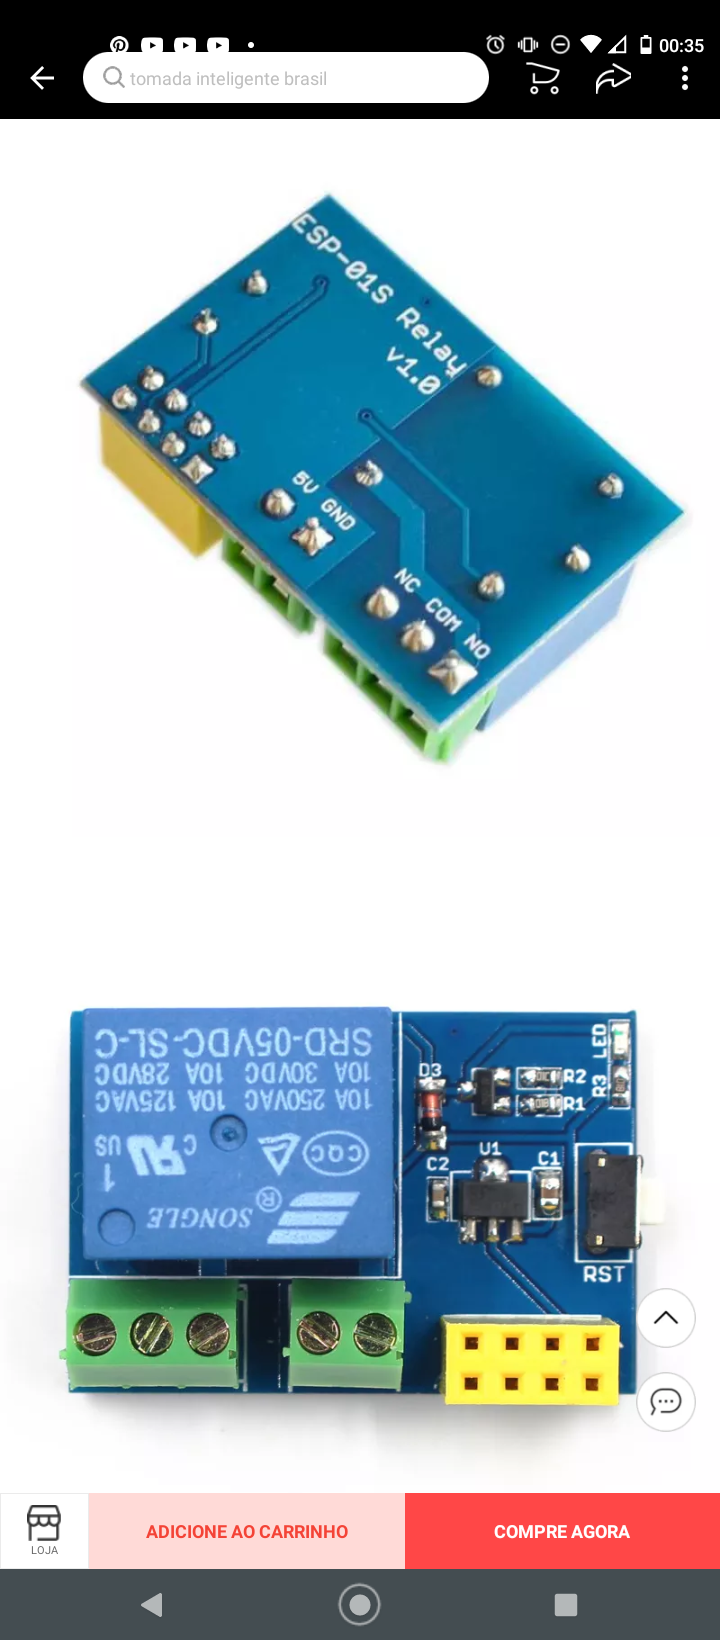
\includegraphics[width=0.7\textwidth]{./module_esp01.png}
\end{figure}

O módulo de relé possui o esquemático como na figura \ref{schematic_relay}
\begin{figure}[h!]
\caption{\label{fig:schematic_relay}Esquema do circuito do módulo com relé}
\centering
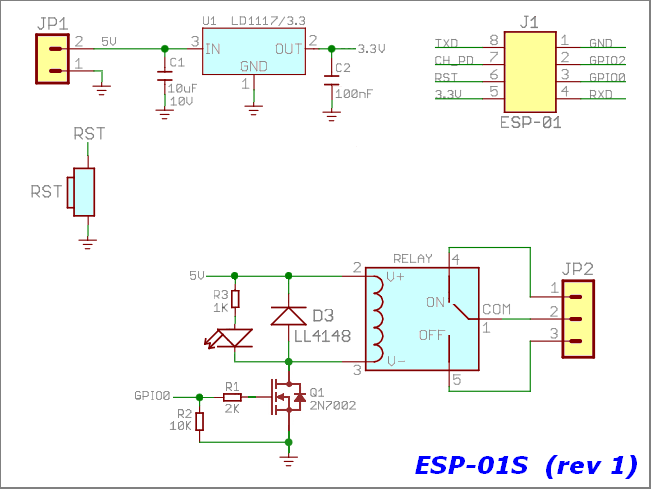
\includegraphics[width=0.7\textwidth]{./schematic_relay.png}
\end{figure}

\subsection{Descrição do software}
\label{sec:org8a2d0fa}
O projeto de software é dividor em 3 partes: Conectividade e gerenciamento de ações; GUI; geração de relatórios
\subsubsection{Conectividade e gerenciamento de ações}
\label{sec:org1f206be}
Esta parte consiste em fazer os ESP8266 se conectarem com o raspberryPI por rede para estabelecer comunicação (vide figura \ref{fig:lan_concept}) e também consiste nas tomadas de decisão para o raspberryPI, determinando o comportamento de cada lâmpada e dando prioridade aos comandos.
Os esp8266 das tomadas devem entrar em um ponto de acesso central e então ficar à espera de comandos. Ele age como escravo para responder aos comandos do computador central.

\begin{figure}[h!]
\caption{\label{fig:lan_concept}Visão conceitual para conectividade LAN dos dispositivos}
\centering
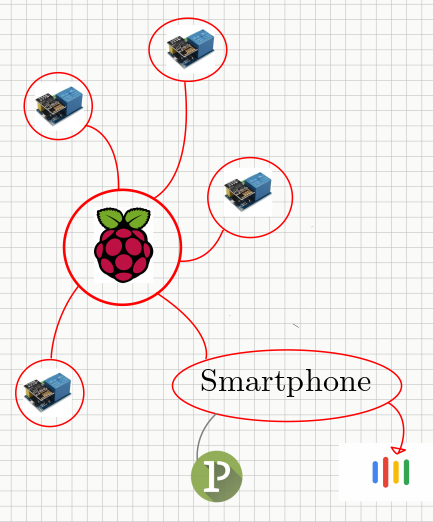
\includegraphics[width=0.7\textwidth]{./lan_concept.png}
\end{figure}

\begin{itemize}
\item Atividades de pesquisa e implementação:
\begin{itemize}
\item Protocolo de comunicação (http)
\begin{itemize}
\item Usar os esps como servidores, de modo que o raspberry consiga solicitar informações.
\end{itemize}
\item Secure shell (ssh) para compartilhar tela
\item Programação dos ESP8266
\begin{itemize}
\item frameworks: Arduino, micropython, RTOS?
\end{itemize}
\end{itemize}
\item Procedimentos a serem utilizados na cpu principal:
\begin{itemize}
\item get state() \# Retorna o estado atual lâmpada;
\item turn(boolean state) \# Pede para ligar/desligar a lâmpada
\item get switch() \# Retorna a posição do interruptor;
\end{itemize}
\end{itemize}

\begin{figure}[h!]
\caption{\label{fig:caso_de_uso}Diagrama de caso de uso}
\centering
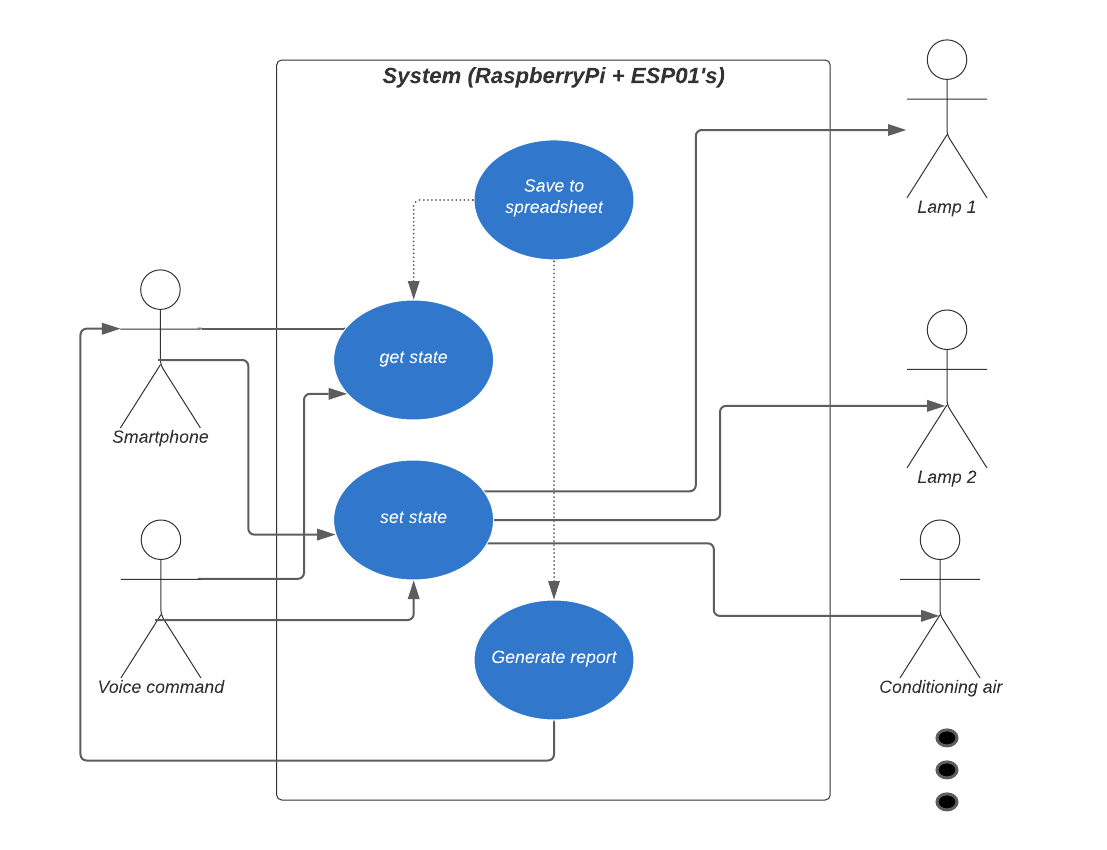
\includegraphics[width=\textwidth]{diagrama_uso.png}
\end{figure}


\subsubsection{GUI}
\label{sec:org7b097fe}
Uma interface gráfica para o usuário como a da figura \ref{fig:gui} é tida como meio de centralizar as informações de forma que fique acessível ao usuário. Esta será feita no raspberryPI IOs com a biblioteca Qt for python, que é uma versão alternativa ao PyQt com licensa LGPL, para caso o projeto futuramente se torne comercial.
\begin{figure}[h!]
\caption{\label{fig:gui}GUI a ser implementada no RaspberryPI OS}
\centering
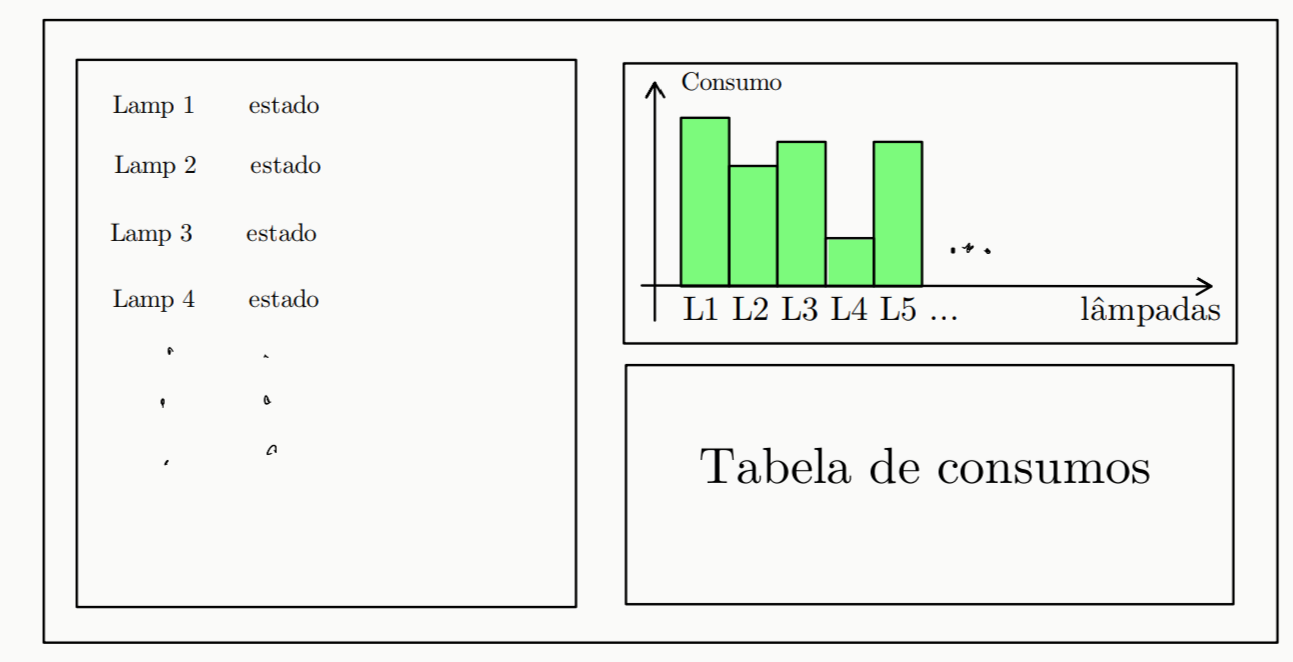
\includegraphics[width=\textwidth]{./gui.png}
\end{figure}

\begin{itemize}
\item Atividades de pesquisa e implementação
TODO!!!
\end{itemize}

\subsubsection{Geração de relatórios}
\label{sec:org91d86b4}
Esta parte do projeto consiste em trabalhar com as informações obtidas com as lâmpadas, visa calcular consumos e gerar um histrograma para o consumo de energia dos dispositivos.

\begin{itemize}
\item Atividades de pesquisa e implementação
TODO!!!
\end{itemize}
\end{document}
